\documentclass[12pt]{article}
\usepackage{amsmath}
\usepackage{amssymb}
\usepackage{geometry}
\usepackage{graphicx}
\usepackage{hyperref}
\usepackage{tikz}
\usepackage{tikz-3dplot}
\usetikzlibrary{arrows.meta, calc, decorations.markings, positioning}

\geometry{margin=1in}

\title{Equations of Motion: 2D Cart + 3D Pendulum System}
\author{Derived from Pendulum3D Class}
\date{\today}

\begin{document}

\maketitle

\section{System Description}

\begin{itemize}
    \item \textbf{Cart}: mass $M$, can translate in 2D ($x$-$y$ plane)
    \item \textbf{Pendulum}: mass $m$, length $L$, attached to cart via 2-DOF gimbal
    \begin{itemize}
        \item \textbf{Gimbal}: $Y$-axis rotation (pitch $\theta$) $\rightarrow$ $X$-axis rotation (roll $\phi$)
    \end{itemize}
\end{itemize}

\section{Reference Frames}

The system uses multiple coordinate frames for the derivation:

\subsection{Frame Definitions}

\begin{enumerate}
    \item \textbf{World Frame (W)}: Inertial reference frame
    \begin{itemize}
        \item Origin: Fixed in space
        \item Axes: $\hat{x}_W$ (left), $\hat{y}_W$ (into page/forward), $\hat{z}_W$ (down)
        \item Right-handed coordinate system
    \end{itemize}
    
    \item \textbf{Cart Frame (C)}: Translates with the cart
    \begin{itemize}
        \item Origin: Cart center of mass at $(x_c, y_c, 0)$
        \item Axes: Parallel to world frame (no rotation)
        \item Translation: $\mathbf{r}_{W,C} = [x_c, y_c, 0]^T$
    \end{itemize}
    
    \item \textbf{Pivot Frame (P)}: Fixed to cart at pendulum attachment point
    \begin{itemize}
        \item Origin: Pendulum attachment point on cart (top of cart)
        \item Axes: Parallel to cart frame (no relative rotation)
        \item This is where the gimbal mechanism is mounted
    \end{itemize}
    
    \item \textbf{Gimbal1 Frame (G1)}: Rotated by pitch angle $\theta$
    \begin{itemize}
        \item Origin: Same as pivot frame
        \item Rotation: $\theta$ about $\hat{y}_P$ (Y-axis, pitch)
        \item Axes after rotation: $\mathbf{R}_y(\theta)$
    \end{itemize}
    
    \item \textbf{Ball Frame (B)}: Rotated by roll angle $\phi$
    \begin{itemize}
        \item Origin: Same as pivot frame
        \item Rotation: $\phi$ about $\hat{x}_{G1}$ (X-axis of gimbal1, roll)
        \item Total rotation from pivot: $\mathbf{R}(\theta, \phi) = \mathbf{R}_x(\phi) \cdot \mathbf{R}_y(\theta)$
    \end{itemize}
\end{enumerate}

\subsection{Frame Transformation Sequence}

The transformation from world frame to ball frame follows:
\begin{equation}
    W \xrightarrow{\text{translate}} C \xrightarrow{\text{translate}} P \xrightarrow{\text{rotate } \theta} G1 \xrightarrow{\text{rotate } \phi} B
\end{equation}

\subsection{System Diagram}

\begin{figure}[h]
\centering
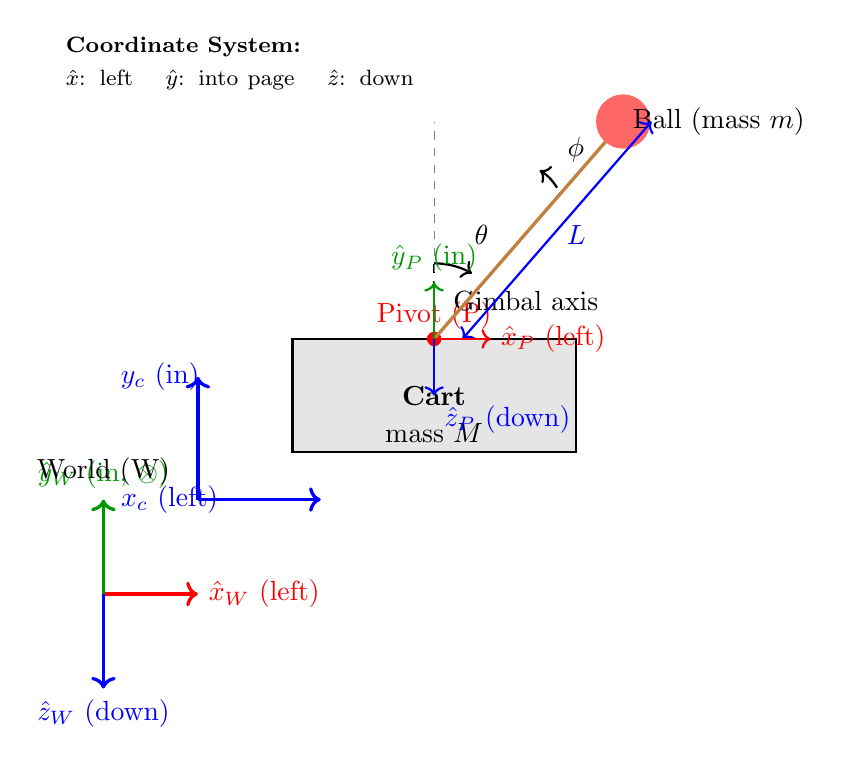
\begin{tikzpicture}[scale=1.2]
    
    % Note about coordinate system
    \node[anchor=north west, text width=5cm] at (-4, 4.5) {
        \footnotesize \textbf{Coordinate System:} \\
        $\hat{x}$: left \quad $\hat{y}$: into page \quad $\hat{z}$: down
    };
    
    % Draw cart (top view in x-y plane)
    \draw[thick, fill=gray!20] (-1.5, 0) rectangle (1.5, 1.2);
    \node at (0, 0.6) {\textbf{Cart}};
    \node at (0, 0.2) {mass $M$};
    
    % Cart position label
    \draw[->, very thick, blue] (-2.5, -0.5) -- (-1.2, -0.5);
    \node[blue] at (-2.8, -0.5) {$x_c$ (left)};
    \draw[->, very thick, blue] (-2.5, -0.5) -- (-2.5, 0.8);
    \node[blue] at (-2.9, 0.8) {$y_c$ (in)};
    
    % Pivot point
    \filldraw[red] (0, 1.2) circle (2pt);
    \node[red, above] at (0, 1.2) {Pivot (P)};
    
    % Gimbal representation
    \draw[thick, dashed] (0, 1.2) -- (0, 2.0);
    \node[right] at (0.1, 1.6) {Gimbal axis};
    
    % Pendulum rod at angle
    \coordinate (pivot) at (0, 1.2);
    \coordinate (gimbal) at (1.2, 2.5);
    \coordinate (ball) at (2.0, 3.5);
    
    \draw[very thick, brown] (pivot) -- (ball);
    \draw[dashed, gray] (pivot) -- (0, 3.5);
    
    % Angle theta (pitch)
    \draw[->, thick] (0, 2.0) arc (90:60:0.8);
    \node at (0.5, 2.3) {$\theta$};
    
    % Angle phi (roll) - shown as rotation around pendulum
    \draw[->, thick] (1.3, 2.8) arc (30:60:0.5);
    \node at (1.5, 3.2) {$\phi$};
    
    % Ball
    \filldraw[red!60] (ball) circle (8pt);
    \node[right] at (ball) {Ball (mass $m$)};
    
    % Length L
    \draw[<->, thick, blue] (0.3, 1.2) -- (2.3, 3.5);
    \node[blue, right] at (1.3, 2.3) {$L$};
    
    % Reference frames at pivot
    \draw[->, thick, red] (0, 1.2) -- (0.6, 1.2) node[right] {$\hat{x}_P$ (left)};
    \draw[->, thick, green!60!black] (0, 1.2) -- (0, 1.8) node[above] {$\hat{y}_P$ (in)};
    \draw[->, thick, blue] (0, 1.2) -- (0, 0.6) node[below right] {$\hat{z}_P$ (down)};
    
    % World frame at origin
    \draw[->, very thick, red] (-3.5, -1.5) -- (-2.5, -1.5) node[right] {$\hat{x}_W$ (left)};
    \draw[->, very thick, green!60!black] (-3.5, -1.5) -- (-3.5, -0.5) node[above] {$\hat{y}_W$ (in, $\otimes$)};
    \draw[->, very thick, blue] (-3.5, -1.5) -- (-3.5, -2.5) node[below] {$\hat{z}_W$ (down)};
    \node at (-3.5, -0.2) {World (W)};
    
\end{tikzpicture}
\caption{2D Cart + 3D Pendulum System (Spherical Coordinates). The cart can translate in the horizontal $x$-$y$ plane. The pendulum hangs down (positive $z$-direction) and its orientation is described by spherical coordinates: $\theta$ (polar angle from $z$-axis) and $\phi$ (azimuthal angle from $x$-axis in the $xy$-plane projection). Coordinate system: $\hat{x}$ left, $\hat{y}$ into page, $\hat{z}$ down.}
\label{fig:system}
\end{figure}

\subsection{Rotation Sequence (Spherical Coordinates)}

In spherical coordinates, the unit vector pointing from the pivot to the ball is given directly by:

\begin{equation}
    \hat{\mathbf{r}} = 
    \begin{bmatrix}
        \sin\theta\cos\phi \\
        \sin\theta\sin\phi \\
        \cos\theta
    \end{bmatrix}
\end{equation}

where:
\begin{itemize}
    \item $\theta$ is the polar angle measured from the $+z$ axis (down)
    \item $\phi$ is the azimuthal angle measured from the $+x$ axis in the $xy$-plane
\end{itemize}

\textbf{Physical interpretation}:
\begin{align}
    \theta &= 0 \quad &\Rightarrow \quad &\hat{\mathbf{r}} = [0, 0, 1]^T \quad &\text{(pointing straight down)} \\
    \theta &= \pi/2, \phi = 0 \quad &\Rightarrow \quad &\hat{\mathbf{r}} = [1, 0, 0]^T \quad &\text{(pointing left)} \\
    \theta &= \pi/2, \phi = \pi/2 \quad &\Rightarrow \quad &\hat{\mathbf{r}} = [0, 1, 0]^T \quad &\text{(pointing into page)} \\
    \theta &= \pi \quad &\Rightarrow \quad &\hat{\mathbf{r}} = [0, 0, -1]^T \quad &\text{(pointing up, inverted)}
\end{align}

\textbf{Spherical basis vectors}:

The natural basis vectors in spherical coordinates are:
\begin{align}
    \hat{\boldsymbol{\theta}} &= \frac{\partial \hat{\mathbf{r}}}{\partial \theta} = 
    \begin{bmatrix}
        \cos\theta\cos\phi \\
        \cos\theta\sin\phi \\
        -\sin\theta
    \end{bmatrix}
    \quad \text{(direction of increasing $\theta$)} \\
    \hat{\boldsymbol{\phi}} &= \frac{1}{\sin\theta}\frac{\partial \hat{\mathbf{r}}}{\partial \phi} = 
    \begin{bmatrix}
        -\sin\phi \\
        \cos\phi \\
        0
    \end{bmatrix}
    \quad \text{(direction of increasing $\phi$)}
\end{align}

\textbf{Important}: The order matters! This is an \textit{intrinsic} rotation sequence (Y-then-X), which is different from Z-Y-X Euler angles (roll-pitch-yaw).

\section{Generalized Coordinates}

The system has 4 degrees of freedom using spherical coordinates for the pendulum:
\begin{equation}
    \mathbf{q} = \begin{bmatrix} x_c \\ y_c \\ \theta \\ \phi \end{bmatrix}
\end{equation}

where:
\begin{itemize}
    \item $x_c, y_c$: Cart position in horizontal plane
    \item $\theta$: Polar angle from $z$-axis (zenith angle), $\theta \in [0, \pi]$
    \begin{itemize}
        \item $\theta = 0$: pendulum points straight down (along $+z$)
        \item $\theta = \pi/2$: pendulum horizontal
        \item $\theta = \pi$: pendulum points up
    \end{itemize}
    \item $\phi$: Azimuthal angle from $x$-axis in $xy$-plane, $\phi \in [0, 2\pi)$
    \begin{itemize}
        \item $\phi = 0$: pendulum projects onto $+x$ axis
        \item $\phi = \pi/2$: pendulum projects onto $+y$ axis
    \end{itemize}
\end{itemize}

\textbf{Note}: This is the standard spherical coordinate parameterization, different from Euler angles.

\section{Kinematics}

\subsection{Cart Position}
\begin{equation}
    \mathbf{r}_{\text{cart}} = \begin{bmatrix} x_c \\ y_c \\ 0 \end{bmatrix}
\end{equation}

\subsection{Pendulum Ball Position}

The ball position relative to the cart (pivot at cart) in spherical coordinates:
\begin{equation}
    \mathbf{r}_{\text{ball}} = \mathbf{r}_{\text{cart}} + L
    \begin{bmatrix}
        \sin\theta\cos\phi \\
        \sin\theta\sin\phi \\
        \cos\theta
    \end{bmatrix}
\end{equation}

where the unit vector in spherical coordinates is:
\begin{equation}
    \hat{\mathbf{r}} = 
    \begin{bmatrix}
        \sin\theta\cos\phi \\
        \sin\theta\sin\phi \\
        \cos\theta
    \end{bmatrix}
\end{equation}

\subsection{Ball Position Components}
\begin{align}
    x_{\text{ball}} &= x_c + L\sin\theta\cos\phi \\

Taking time derivatives of the ball position:
\begin{align}
    \dot{x}_{\text{ball}} &= \dot{x}_c + L(\dot{\theta}\cos\theta\cos\phi - \dot{\phi}\sin\theta\sin\phi) \\
    \dot{y}_{\text{ball}} &= \dot{y}_c + L(\dot{\theta}\cos\theta\sin\phi + \dot{\phi}\sin\theta\cos\phi) \\
    \dot{z}_{\text{ball}} &= -L\dot{\theta}\sin\theta
\end{align}

The velocity magnitude squared:
\begin{align}
    \dot{\mathbf{r}}_{\text{ball}}^2 &= \dot{x}_{\text{ball}}^2 + \dot{y}_{\text{ball}}^2 + \dot{z}_{\text{ball}}^2 \nonumber \\
    &= \dot{x}_c^2 + \dot{y}_c^2 + L^2(\dot{\theta}^2 + \dot{\phi}^2\sin^2\theta) \nonumber \\
    &\quad + 2L(\dot{x}_c\dot{\theta}\cos\theta\cos\phi - \dot{x}_c\dot{\phi}\sin\theta\sin\phi) \nonumber \\
    &\quad + 2L(\dot{y}_c\dot{\theta}\cos\theta\sin\phi + \dot{y}_c\dot{\phi}\sin\theta\cos\phi)
\textbf{Physical interpretation}:
\begin{itemize}
    \item When $\theta = 0$: ball hangs straight down at $(x_c, y_c, L)$
    \item When $\theta = \pi/2, \phi = 0$: ball is horizontal along $+x$ at $(x_c + L, y_c, 0)$
    \item When $\theta = \pi/2, \phi = \pi/2$: ball is horizontal along $+y$ at $(x_c, y_c + L, 0)$
\end{itemize}

\subsection{Ball Velocity (Time Derivatives)}
\begin{align}
    \dot{x}_{\text{ball}} &= \dot{x}_c - L\dot{\theta}\cos\theta \\
    \dot{y}_{\text{ball}} &= \dot{y}_c + L\dot{\phi}\cos\phi\cos\theta - L\dot{\theta}\sin\phi\sin\theta \\
    \dot{z}_{\text{ball}} &= L\dot{\phi}\sin\phi\cos\theta + L\dot{\theta}\cos\phi\sin\theta
\end{align}

\section{Lagrangian Formulation}

\subsection{Kinetic Energy}

\textbf{Total Kinetic Energy:}
\begin{equation}
    T = T_{\text{cart}} + T_{\text{ball}}
\end{equation}\dot{x}_c^2 + \dot{y}_c^2 + L^2(\dot{\theta}^2 + \dot{\phi}^2\sin^2\theta) \right. \nonumber \\
    &\quad + 2L\dot{x}_c(\dot{\theta}\cos\theta\cos\phi - \dot{\phi}\sin\theta\sin\phi) \nonumber \\
    &\quad \left. + 2L\dot{y}_c(\dot{\theta}\cos\theta\sin\phi + \dot{\phi}\sin\theta\cos\phi)\right]
\end{align}

\textbf{Total Kinetic Energy:}
\begin{align}
    T &= \frac{1}{2}(M + m)(\dot{x}_c^2 + \dot{y}_c^2) + \frac{1}{2}mL^2(\dot{\theta}^2 + \dot{\phi}^2\sin^2\theta) \nonumber \\
    &\quad + mL\dot{x}_c(\dot{\theta}\cos\theta\cos\phi - \dot{\phi}\sin\theta\sin\phi) \nonumber \\
    &\quad + mL\dot{y}_c(\dot{\theta}\cos\theta\sin\phi + \dot{\phi}\sin\theta\cos\phi
\begin{align}
    T_{\text{ball}} &= \frac{1}{2}m\left[\dot{x}_c^2 + \dot{y}_c^2 + L^2\dot{\theta}^2 + L^2\dot{\phi}^2\cos^2\theta \right. \nonumber \\
    &\quad - 2L\dot{x}_c\dot{\theta}\cos\theta + 2L\dot{y}_c\dot{\phi}\cos\phi\cos\theta \nonumber \\
    &\quad \left. - 2L\dot{y}_c\dot{\theta}\sin\phi\sin\theta\right]
\end{align}

\textbf{Total Kinetic Energy:}
\begin{align}
    T &= \frac{1}{2}(M + m)(\dot{x}_c^2 + \dot{y}_c^2) + \frac{1}{2}mL^2(\dot{\theta}^2 + \dot{\phi}^2\cos^2\theta) \nonumber \\
    &\quad - mL\dot{x}_c\dot{\theta}\cos\theta + mL\dot{y}_c(\dot{\phi}\cos\phi\cos\theta - \dot{\theta}\sin\phi\sin\theta)
\end{align}

\subsection{Potential Energy}

With $z$ pointing down, the gravitational potential energy is (taking $V = 0$ at pivot level):
\begin{equation}
    V = -mgz_{\text{ball}} = -mgL\cos\phi\cos\theta
\end{equation}

Note: The negative sign arises because gravity acts in the positive $z$-direction (down), and potential energy decreases as the ball goes down.
sin^2\theta) \nonumber \\
    &\quad + mL\dot{x}_c(\dot{\theta}\cos\theta\cos\phi - \dot{\phi}\sin\theta\sin\phi) \nonumber \\
    &\quad + mL\dot{y}_c(\dot{\theta}\cos\theta\sin\phi + \dot{\phi}\sin\theta\cos\phi) \nonumber \\
    &\quad + mgL
    \mathcal{L} &= T - V \nonumber \\
    &= \frac{1}{2}(M + m)(\dot{x}_c^2 + \dot{y}_c^2) + \frac{1}{2}mL^2(\dot{\theta}^2 + \dot{\phi}^2\cos^2\theta) \nonumber \\
    &\quad - mL\dot{x}_c\dot{\theta}\cos\theta + mL\dot{y}_c(\dot{\phi}\cos\phi\cos\theta - \dot{\theta}\sin\phi\sin\theta) \nonumber \\
    &\quad + mgL\cos\phi\cos\theta
\end{align}

\section{Euler-Lagrange Equations}

The equations of motion are derived from:
\begin{equation}
    \frac{d}{dt}\left(\frac{\partial\mathcal{L}}{\partial\dot{q}_i}\right) - \frac{\partial\mathcal{L}}{\partial q_i} = Q_i
\end{equation}

where $Q_i$ are generalized forces (control inputs, friction, etc.).

For this system:
\begin{align}
    Q_{x_c} &= F_x \quad \text{(horizontal force on cart in $x$-direction)} \\
    Q_{y_c} &= F_y \quad \text{(horizontal force on cart in $y$-direction)} \\
    Q_\theta &= \tau_\theta \quad \text{(torque about $Y$-axis / pitch joint)} \\
    Q_\phi &= \tau_\phi \quad \text{(torque about $X$-axis / roll joint)}
\end{align}

\section{Equations of Motion (Compact Form)}
polar axis)} \\
    Q_\phi &= \tau_\phi \quad \text{(torque about azimuthal axis

\begin{equation}
    \mathbf{M}(\mathbf{q}) = 
    \begin{bmatrix}
        M+m & 0 & -mL\cos\theta & mL\cos\phi\cos\theta \\
        0 & M+m & -mL\sin\phi\sin\theta & mL\cos\phi\cos\theta \\
        -mL\cos\theta & -mL\sin\phi\sin\theta & mL^2 & 0 \\
        mL\cos\phi\cos\theta & mL\cos\phi\cos\theta & 0 & mL^2\cos^2\theta
    \end{bmatrix}
\end{equation}mL\cos\theta\cos\phi & -mL\sin\theta\sin\phi \\
        0 & M+m & mL\cos\theta\sin\phi & mL\sin\theta\cos\phi \\
        mL\cos\theta\cos\phi & mL\cos\theta\sin\phi & mL^2 & 0 \\
        -mL\sin\theta\sin\phi & mL\sin\theta\cos\phi & 0 & mL^2\sin^2\theta
    \end{bmatrix}
\end{equation}

Note: The $\phi$-inertia term is $mL^2\sin^2\theta$, which goes to zero at $\theta = 0$ (pendulum hanging down) and is maximum at $\theta = \pi/2$ (horizontal).dot{\theta}^2\sin\theta - mL\dot{\phi}^2\cos\phi\sin\theta\cos\theta \\
    C_2 &= mL\dot{\phi}^2\sin\phi\cos\phi\cos^2\theta + mL\dot{\theta}^2\sin\phi\cos\theta \\
    C_3 &= mL\dot{\phi}^2\sin\theta\cos\theta - mL\dot{y}_c\dot{\phi}\cos\phi\sin\theta \\
    C_4 &= -mL^2\dot{\theta}\dot{\phi}\sin\theta\cos\theta - mL\dot{y}_c\dot{\theta}\cos\phi\sin\theta
With gravity acting in the positive $z$-direction (down):
\end{align}

\subsection{Gravity Vector $\mathbf{G}(\mathbf{q})$}

\begin{align}
    G_1 &= 0 \\
    G_2 &= 0 \\
    G_3 &= -mgL\cos\phi\sin\theta \\
    G_4 &= mgL\sin\phi\cos\theta
\end{align}

\subsection{Control Input Vector}

\begin{equation}
    \mathbf{Q} = \begin{bmatrix} F_x \\ F_y \\ \tau_\theta \\ \tau_\phi \end{bmatrix}
\end{equation}

\subsection{Final Equations of Motion}

\begin{equation}
    \mathbf{M}(\mathbf{q})\ddot{\mathbf{q}} + \mathbf{C}(\mathbf{q},\dot{\mathbf{q}}) + \mathbf{G}(\mathbf{q}) = \mathbf{Q}
\end{equation}

\textbf{Expanded FmL\cos\theta\cos\phi & -mL\sin\theta\sin\phi \\
        0 & M+m & mL\cos\theta\sin\phi & mL\sin\theta\cos\phi \\
        mL\cos\theta\cos\phi & mL\cos\theta\sin\phi & mL^2 & 0 \\
        -mL\sin\theta\sin\phi & mL\sin\theta\cos\phi & 0 & mL^2\sin^2\theta
    \end{bmatrix}
    \begin{bmatrix}
        \ddot{x}_c \\ \ddot{y}_c \\ \ddot{\theta} \\ \ddot{\phi}
    \end{bmatrix}
    +
    \begin{bmatrix}
        C_1 \\ C_2 \\ C_3 \\ C_4
    \end{bmatrix}
    +
    \begin{bmatrix}
        0 \\ 0 \\ -mgL\sin\theta \\ 0
    +
    \begin{bmatrix}
        0 \\ 0 \\ G_3 \\ G_4
    \end{bmatrix}
    =
    \begin{bmatrix}
        F_x \\ F_y \\ \tau_\theta \\ \tau_\phi
    \end{bmatrix}
\end{equation}

\section{Special Cases}

\subsection{Fixed Cart ($x_c =spherical pendulum
    \item Mass matrix becomes diagonal: $\text{diag}(mL^2, mL^2\sin^2\theta)$
    \item Classic problem with conserved angular momentum about vertical axis when $\tau_\phi = 0$
\end{itemize}

\subsection{Small Angles ($\theta \approx 0$)}
\begin{itemize}
    \item $\sin\theta \approx \theta$, $\cos\theta \approx 1$
    \item Pendulum near vertical (hanging down)
    \item Linearized system:
    \begin{align}
        x_{\text{ball}} &\approx x_c + L\theta\cos\phi \\
        y_{\text{ball}} &\approx y_c + L\theta\sin\phi \\
        z_{\text{ball}} &\approx L
    \end{align}
    \item Useful for LQR controller design
\end{itemize}

\subsection{Planar Motion ($\phi = \text{const}$)}
\begin{itemize}
    \item Motion confined to a vertical plane
    \item 3 DOF: $[x_c, y_c, \theta]$
    \item If $\phi = 0$: motion in $x$-$z$ plane
    \item If $\phi = \pi/2$: motion in $y$-$z$ plane
\end{itemize}

\subsection{Equilibrium Points}
\begin{itemize}
    \item \textbf{Stable}: $\theta = 0$ (pendulum hanging down), $\phi$ arbitrary
    \item \textbf{Unstable}: $\theta = \pi$ (inverted pendulum), $\phi$ arbitrary
    \item At $\theta = 0$: Mass matrix becomes singular for $\phi$-coordinate (gimbal lock)
    \item Classical cart-pole problem in 3D
    \item 3 DOF: $[x_c, \theta, \phi]$
\end{itemize}

\section{Usage in Drake}

Drake automatically derives and solves these equations via:
\begin{itemize}
    \item \texttt{MultibodyPlant} with \texttt{SpatialInertia}
    \item \texttt{CalcInverseDynamics(context, vdot, external\_forces)}
    \item \texttt{CalcMassMatrix(context)}
    \item \texttt{CalcBiasTerm(context)} [combines $\mathbf{C}(\mathbf{q},\dot{\mathbf{q}}) + \mathbf{G}(\mathbf{q})$]
\end{itemize}

This document provides the analytical form for:
\begin{itemize}
    \item Controller design
    \item Simulation verification
    \item Educational purposes
    \item Custom dynamics if needed
\end{itemize}

\section{State-Space Representation}

For control design, the system can be represented in state-space form:
\begin{align}
    \mathbf{x} &= \begin{bmatrix} \mathbf{q} \\ \dot{\mathbf{q}} \end{bmatrix} = 
    \begin{bmatrix} x_c \\ y_c \\ \theta \\ \phi \\ \dot{x}_c \\ \dot{y}_c \\ \dot{\theta} \\ \dot{\phi} \end{bmatrix} \quad \text{(8 states)} \\
    \mathbf{u} &= \begin{bmatrix} F_x \\ F_y \\ \tau_\theta \\ \tau_\phi \end{bmatrix} \quad \text{(4 inputs)}
\end{align}

The nonlinear dynamics:
\begin{equation}
    \dot{\mathbf{x}} = 
    \begin{bmatrix}
        \dot{\mathbf{q}} \\
        \mathbf{M}^{-1}(\mathbf{q})[\mathbf{u} - \mathbf{C}(\mathbf{q},\dot{\mathbf{q}}) - \mathbf{G}(\mathbf{q})]
    \end{bmatrix}
\end{equation}

For linearization around equilibrium $(\theta_{\text{eq}}, \phi_{\text{eq}})$ (typically $0, 0$):
\begin{equation}
    \dot{\mathbf{x}} = \mathbf{A}\mathbf{x} + \mathbf{B}\mathbf{u}
\end{equation}

where $\mathbf{A}$ is the $8 \times 8$ state matrix and $\mathbf{B}$ is the $8 \times 4$ input matrix.

\end{document}
